%!TEX root =../quadrotorbook.tex
\chapter{Introduction}
\label{chap:introduction}


The book will be organized around the architecture shown in Figure~\ref{fig:intro_architecture}.

\begin{figure*}[h]
   \centering
   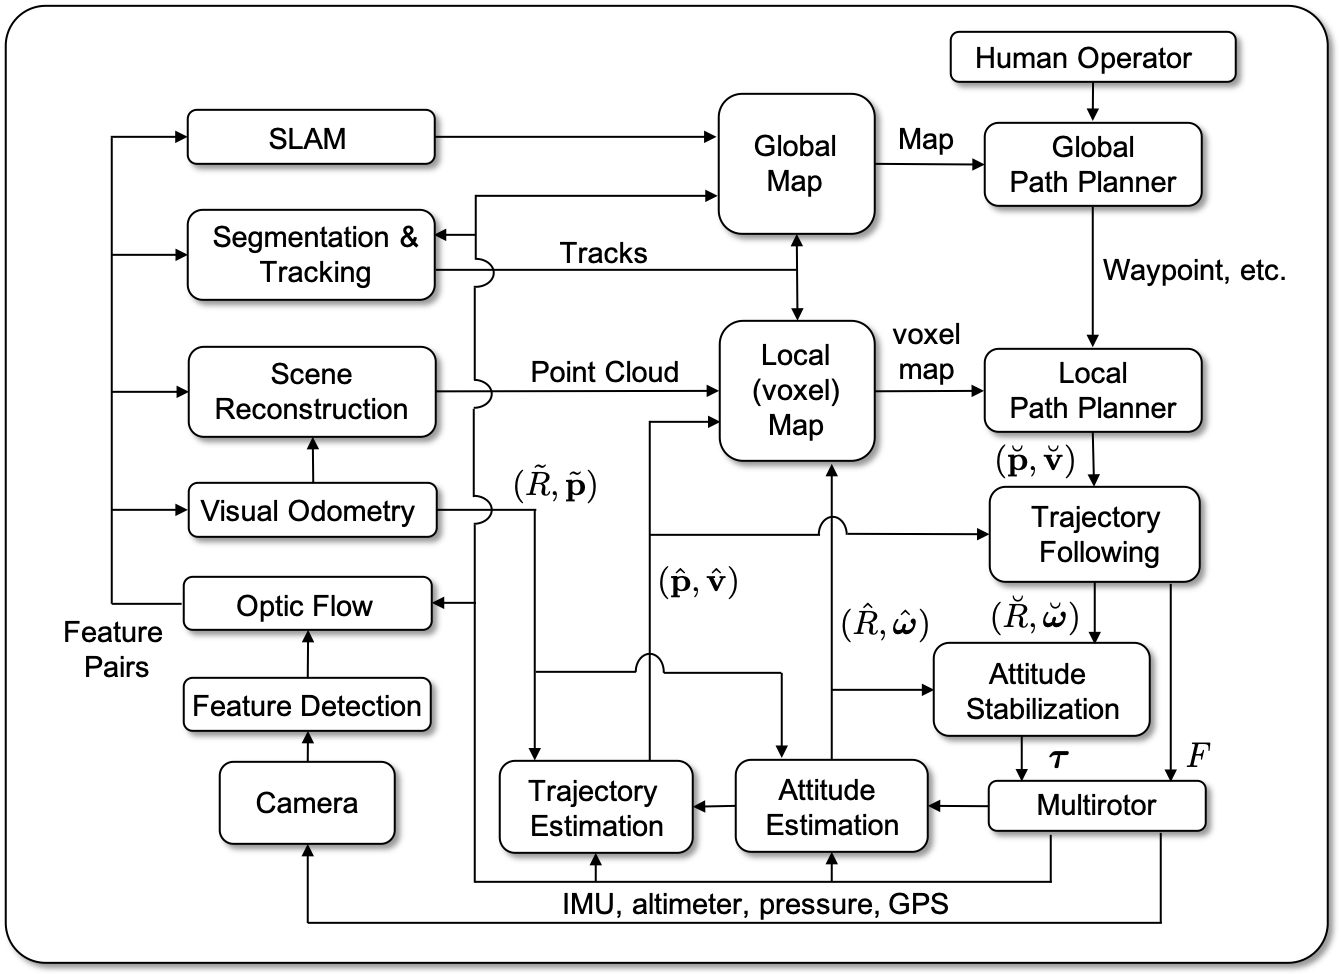
\includegraphics[width=\linewidth]{chap1_intro/figures/architecture} 
   \caption{Software architecture for multirotor estimation and control.}
   \label{fig:intro_architecture}
\end{figure*}

In the bottom right corner is the {\em Multirotor} block representing both the physical flying vehicle and the onboard sensors, including IMU, altimeter, pressure sensors, and possibly a GNSS receiver.  We also assume that the platform has a camera, which we have drawn in its own block.  The equations of motion for the multirotor and the mathematical models for the sensors will be described in Chapter~\ref{chap:multirotor}.  The commanded inputs to the multirotor will be assumed to be the force in the body $z$-axis $F$, and the torque applied to the body $\taubf$.  
%
The {\em Attitude Stabilization} block is discussed in Chapter~\ref{chap:attitude_control}.  In the literature, three different representations for attitude are commonly used, namely Euler angles, quaternions, and rotation matrices.  We will describe attitude stabilization schemes for each representation.  The output of the attitude stabilization block is the applied torque $\taubf$.  The input is the desired attitude $\breve{R}$ and the desired angular rate $\breve{\omegabf}$
%
The {\em Trajectory Following} block is discussed in Chapter~\ref{chap:trajectory_following}.  The input to the trajectory follower is the desired position $\breve{\pbf}$ and the desired velocity $\breve{\vbf}$.  

The second part of the book is concerned with cameras, computer vision, and state estimation.  The {\em Camera} and {\em Feature Detection} blocks shown in Figure~\ref{fig:intro_architecture} are described in Chaper~\ref{chap:camera_features}.  {\em Optical Flow} is discussed in Chapter~\ref{chap:optical_flow}, both how optic flow is computed, as well as how it can be used to navigate a multirotor through urban canyons.  
%
{\em Visual Odometry} is discussed in Chapter~\ref{chap:visual_odometry}.  We then return to the important task of state estimation.  {\em Attitude Estimation} is described in Chapter~\ref{chap:attitude_estimation}, where we include estimation schemes that use feature matching, optic flow, and visual odometry.  In a similar way, {\em Trajectory Estimation} is described in Chapter~\ref{chap:trajectory_estimation}. 

The final part of the book focuses on mapping and planning.  {\em Scene Reconstruction} using a {\em Local Voxel Map} is detailed in Chapter~\ref{chap:scene_reconstruction}.  {\em Segmentation and Tracking} is discussed in Chapter~\ref{chap:tracking}.  The {\em Local Path Planner} is then described in Chapter~\ref{chap:local_planner} where we describe differential flatness, spline-based planning, and visual servoing.  One particular implementation of Simultaneous Localization and Mapping ({\em SLAM}) is then described in Chapter~\ref{chap:SLAM}, and global path planning using the global map created by SLAM is described in Chapter~\ref{chap:global_planner}.





